\section{Administrationshandbuch}
Hier wird mit Beispielbildern erklärt, wie die Software bedient wird und was der Benutzer alles 
in der Software ausführen kann.

\subsection{Chat}
Den Chat kann man mit localhost:4200/chat erreichen. Wenn localhost:4200
eingegeben wird, wird der Benutzer zu der Adresse vom chat weitergeleitet.
An der Seite angekommen kann der Nutzer dann mit dem ChatBot schreiben. 
Der Benutzer kann mit dem ChatBot interagieren indem er eine Frage in dem Textfeld schreibt
und dann mit dem Sendebutton versendet.

\subsection{Admininterface}
Das Admininterface ist nur für Admins erreichbar mit localhost:4200/admin-interface. Der Admin muss sich per Keycloak
anmelden und wird erst dann weitergeleitet zum Bearbeiten der verschiednen Funktionen
des Chatbots.
Nach dem Anmelden mit Kezcloak wird der Benutzer zur Infopage Seite weitergeleitet.
welche mit der Adresse localhost:4200/admin-interface/infopage gekennzeichnet ist.

\subsubsection{Allgemein}
Das Allgemein ist für den Admin erreichber mit localhost:4200/admin-interface/allgemein. 
Der Admin kann dort den Bot Avatar ändern diese wird dann auch im chat geändert.

\subsubsection{Korpus}
Der Korpus ist für den Admin erreichbar mit localhost:4200/admin-interface/corpus.]
Im Korpus kann der Admin einen neuen Intent hinzufügen und auch diese Entfernen. 
Er kann außerdem auch Fragen, die er den Bot stellen will erstellen und auch die 
dazugehörige Antwort hinzufügen.

\subsubsection{Einstellungen}
Der Einstellungsbereich ist für den Admin zugänglich mit der Adresse 
localhost:4200/admin-interface/einstellungen.
Hier kann der Admin seine Domänen zu den Gruppen hinzufügen. Die Korpusdaten, die zugeteilt sind,
können nur von der Gruppe benutzt werden, welche diese zugeteilt bekommen hat. 
Zum Beispiel kann ein nicht registrierter Nutzer nur die Basis Korpusdaten einsehen und nicht die von der Hochschule.

\subsubsection{Keycloak}
Die Admininstrations Console von Keycloak ist erreichbar mit http://localhost:8080. 

\begin{figure}[H]
    \centering
    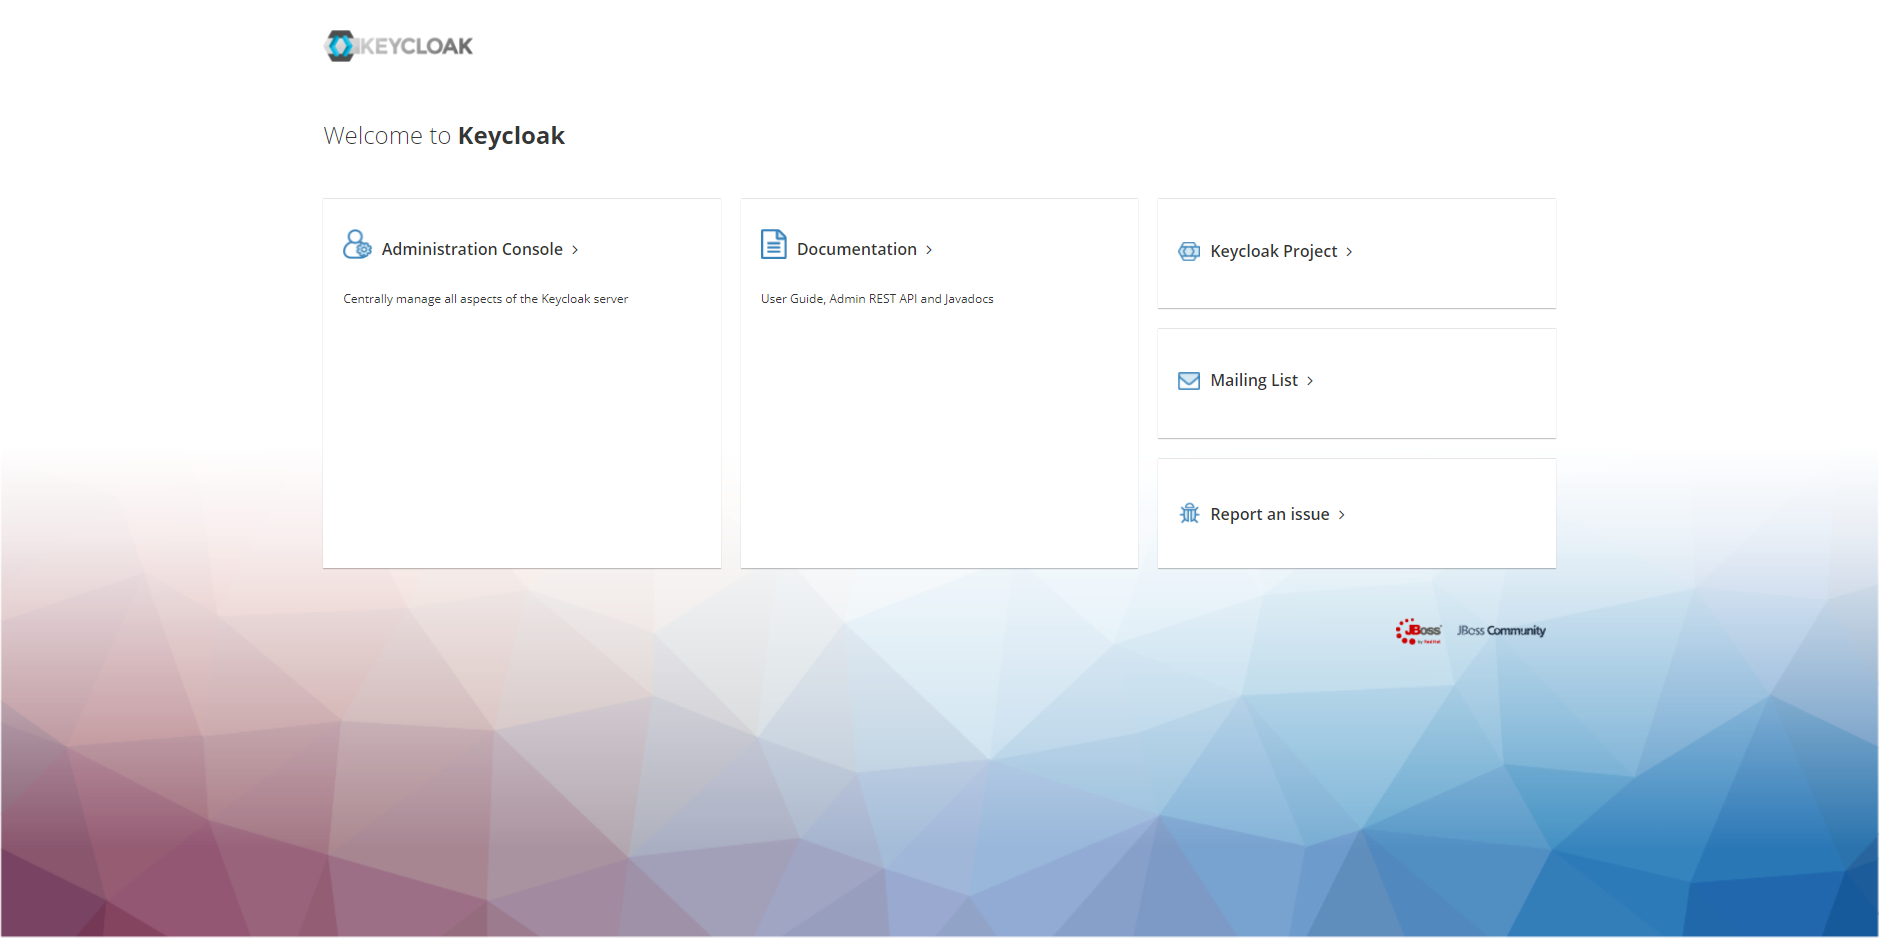
\includegraphics[width=1.0\textwidth]{bilder/administrationshandbuch/keycloak_startseite.png}
    \caption{Keycloak Startseite}
    \label{fig:Keycloak_Startseite}
\end{figure}

\noindent Über einen Klick auf die Schaltfläche ''Admininstration Console'' kommt man zu einem Login-Screen.
Die Daten für den Admin-Login lauten: 
\begin{itemize}
    \item Username: admin
    \item Password: admin
\end{itemize}

\noindent Nach dem Login sollte man sicherstellen, dass oben links der Realm ''QuestMe'' eingestellt ist 
und nicht ''Master''. Der Master-Realm sollte nicht Bearbeitet werden. 
Zum wechseln des Reamls einfach über die Schaltfläche fahren und über das Dropdown-Menü den richtigen Realm auswählen. 

\begin{figure}[H]
    \centering
    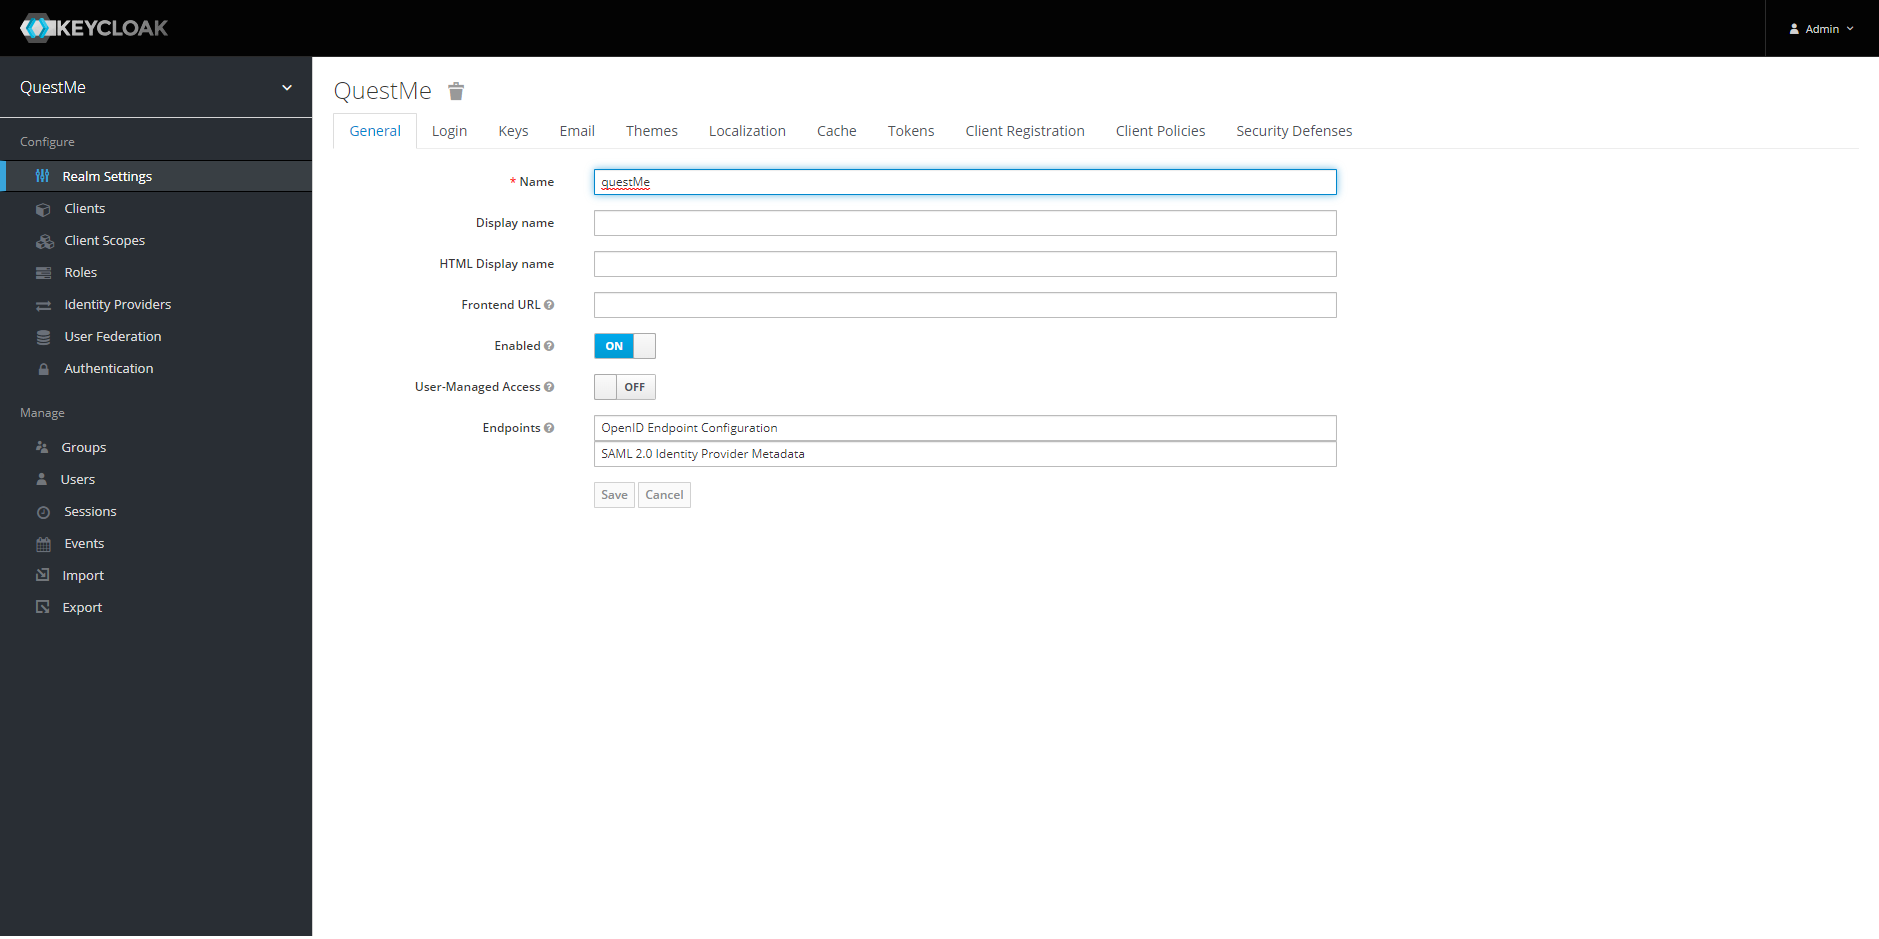
\includegraphics[width=1.0\textwidth]{bilder/administrationshandbuch/keycloak_nach_login.png}
    \caption{Keycloak Übersicht}
    \label{fig:Keycloak_Uebersicht}
\end{figure}

\noindent Durch einen Klick auf die Schaltfläche ''Clients'' kommt man zu den Client-Konfigurationen. 
Der Client ''questMe-openid-client'' ist für das Frontend und der Client ''questMe-openid-rest-client'' ist für das Backend. 

\begin{figure}[H]
    \centering
    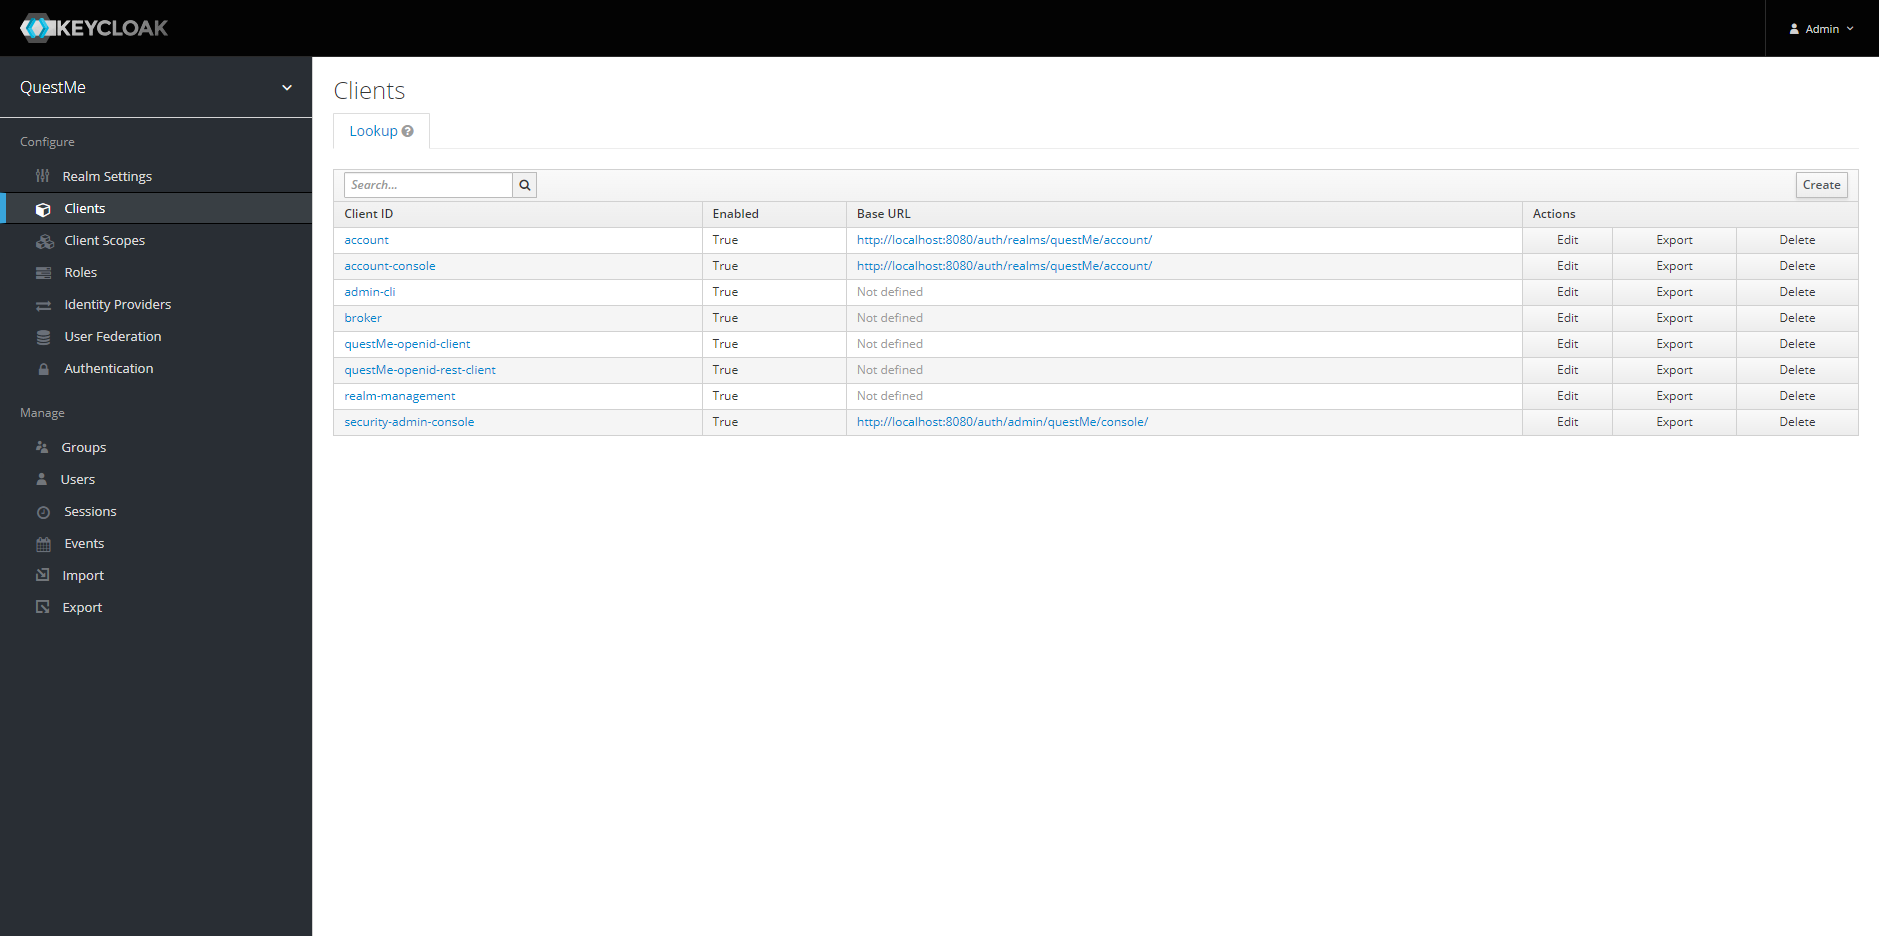
\includegraphics[width=1.0\textwidth]{bilder/administrationshandbuch/keycloak_clients.png}
    \caption{Keycloak Clients}
    \label{fig:Keycloak_Clients}
\end{figure}

\noindent Wenn man einen Client ausgewählt hat, kann man über den oberen Button ''Roles'', nicht den an der Seite, 
sich die Client-Rollen anzeigen lassen.

\begin{figure}[H]
    \centering
    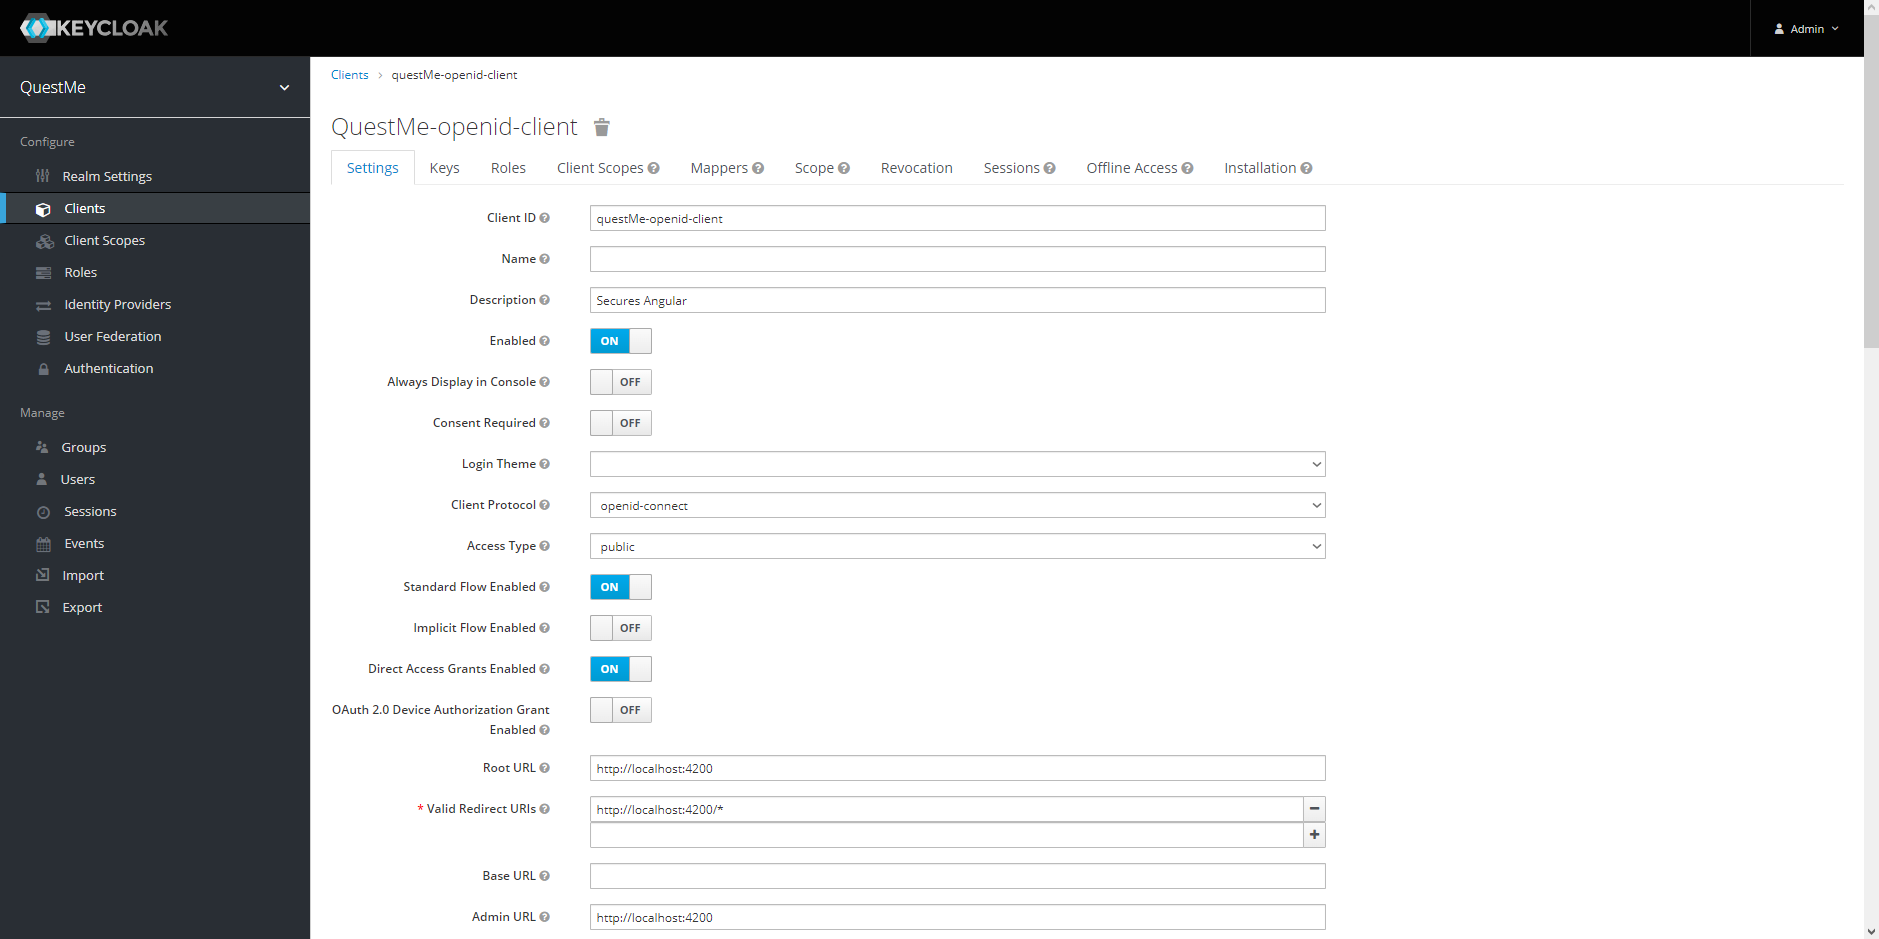
\includegraphics[width=1.0\textwidth]{bilder/administrationshandbuch/keycloak_client_selected.png}
    \caption{Keycloak Client ausgewählt}
    \label{fig:Keycloak_Client_ausgewaehlt}
\end{figure}

\noindent Klickt man auf den ''Roles'' Button an der Seite, kann man die Realm-Rollen einsehen.

\begin{figure}[H]
    \centering
    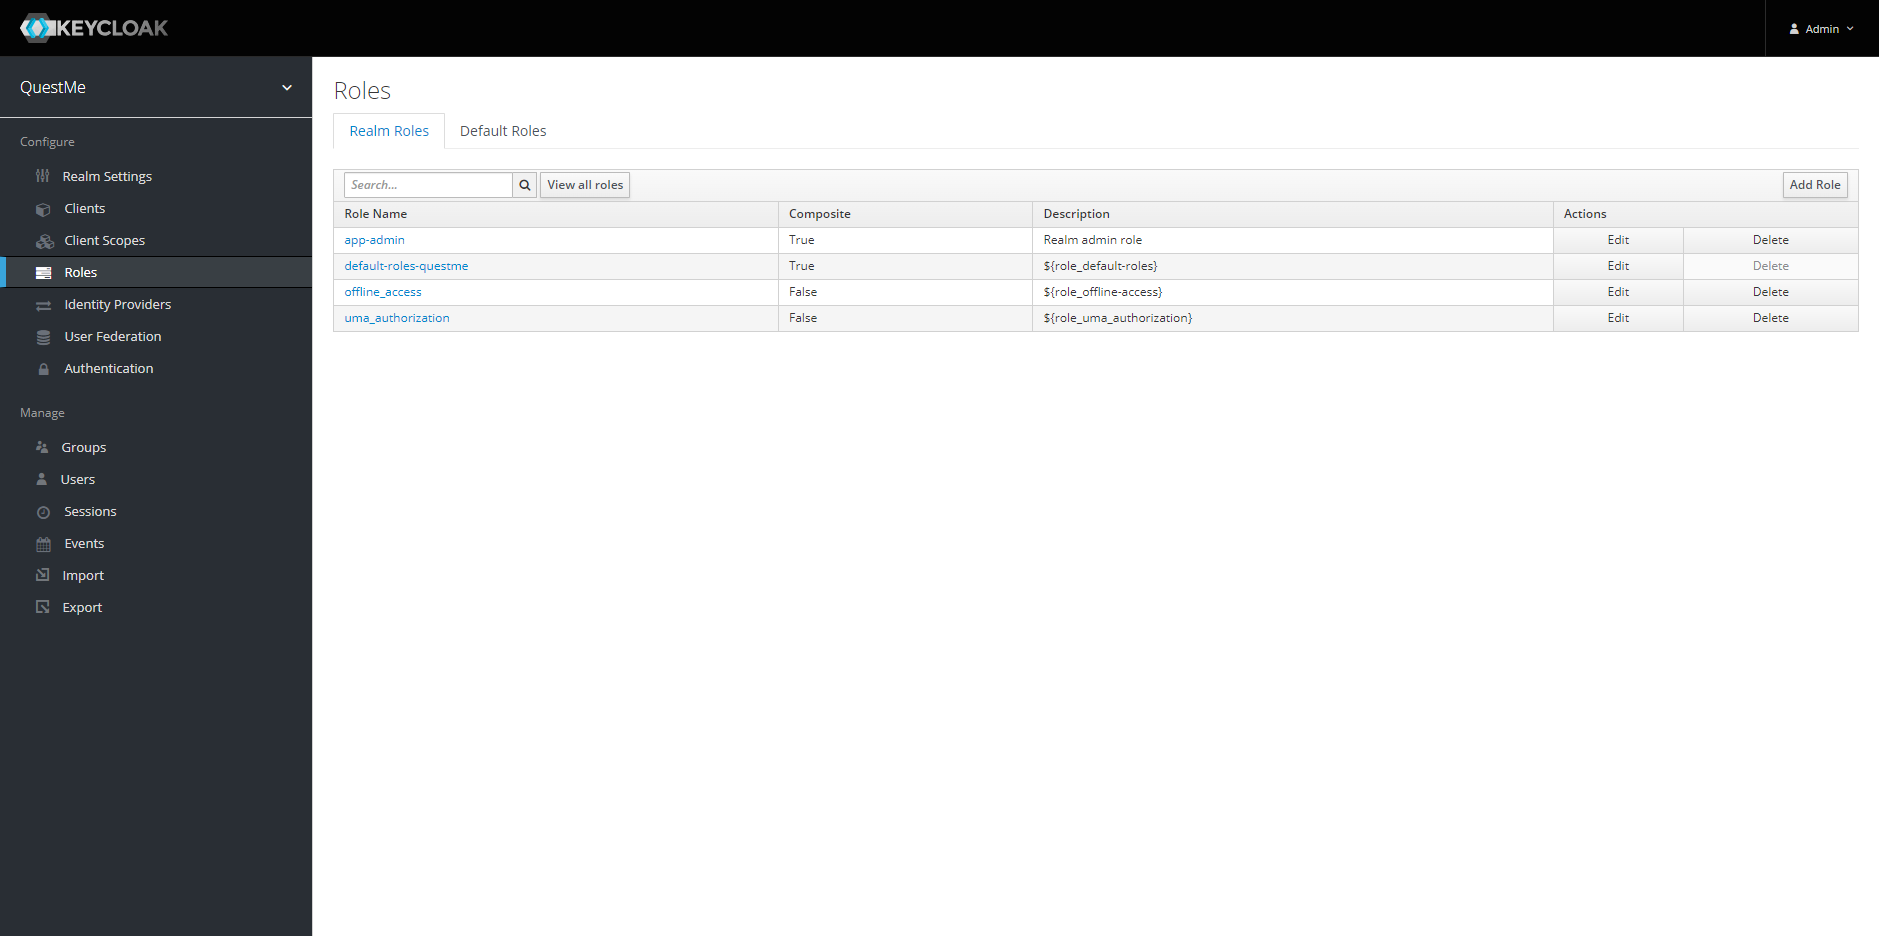
\includegraphics[width=1.0\textwidth]{bilder/administrationshandbuch/keycloak_realm_roles.png}
    \caption{Keycloak Realm-Rollen}
    \label{fig:Keycloak_Realm_Rollen}
\end{figure}

\noindent Unter Client Scopes, links an der Seite, findet man den Scope ''client-roles-questMe-app''. 
Dieser wird benötigt, dass die Nutzerrollen im Token gespeichert werden.

\begin{figure}[H]
    \centering
    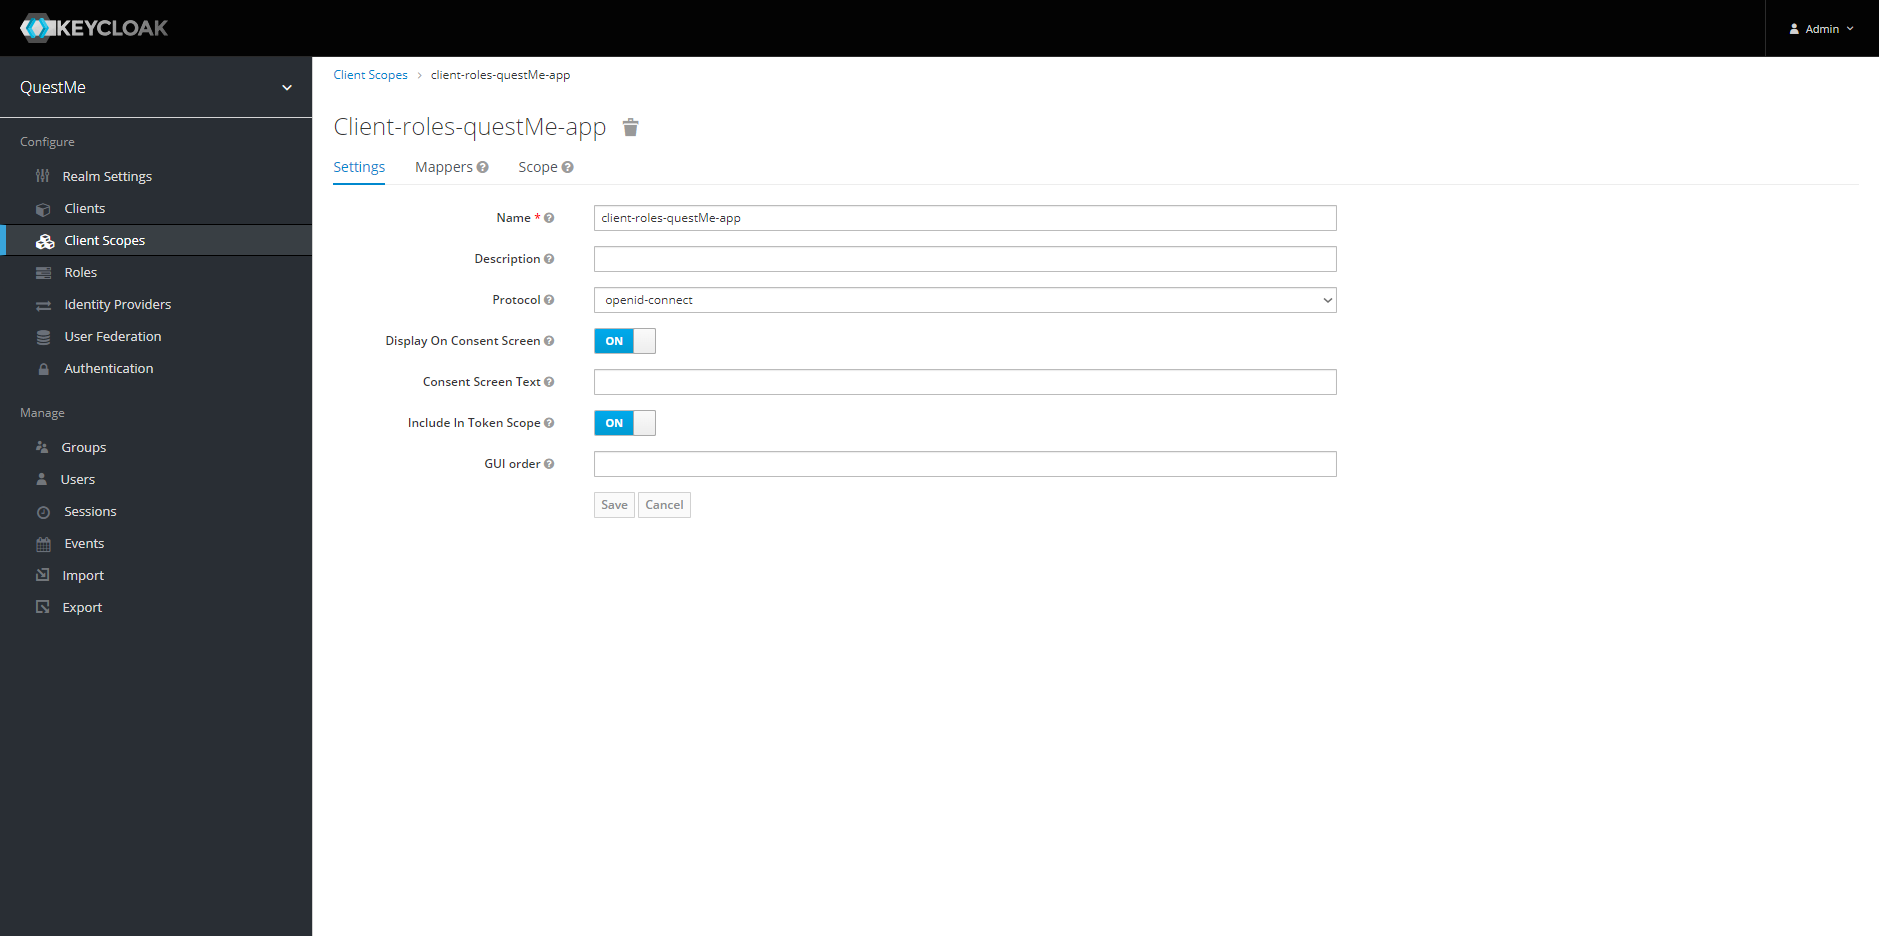
\includegraphics[width=1.0\textwidth]{bilder/administrationshandbuch/keycloak_client_scope.png}
    \caption{Keycloak Client-Scope}
    \label{fig:Keycloak_Client_Scope}
\end{figure}

\noindent Durch einen Klick auf den Button ''Users'' an der linken Seite, kann man alle Nutzer einsehen. 
Damit diese angezeigt werden, muss man zuerst noch auf ''View all users'' klicken.

\begin{figure}[H]
    \centering
    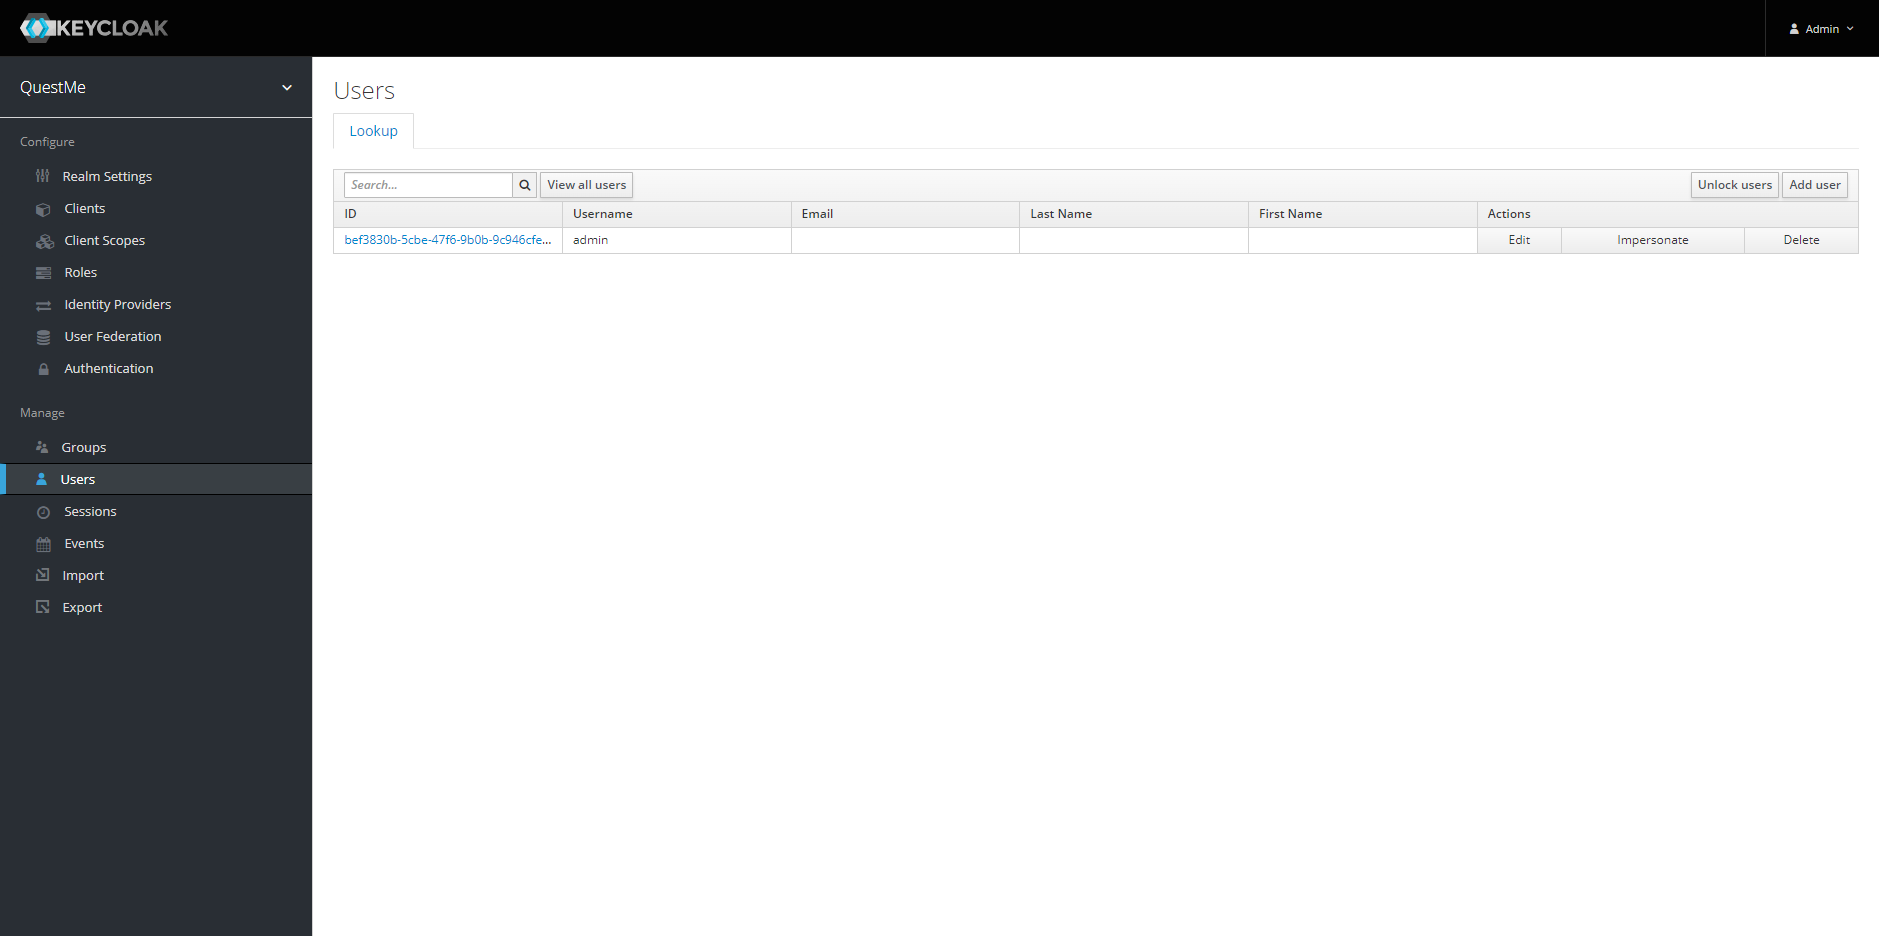
\includegraphics[width=1.0\textwidth]{bilder/administrationshandbuch/keycloak_users.png}
    \caption{Keycloak Users}
    \label{fig:Keycloak_Users}
\end{figure}

\noindent Wenn man einen User bearbeitet, kann man unter dem Unterpunkt ''Role Mappings'' die Rollen des Nutzers einsehen. 
Um die Client-Rollen zu sehen, muss über das Dropdown-Menü ein Client ausgewählt werden.

\begin{figure}[H]
    \centering
    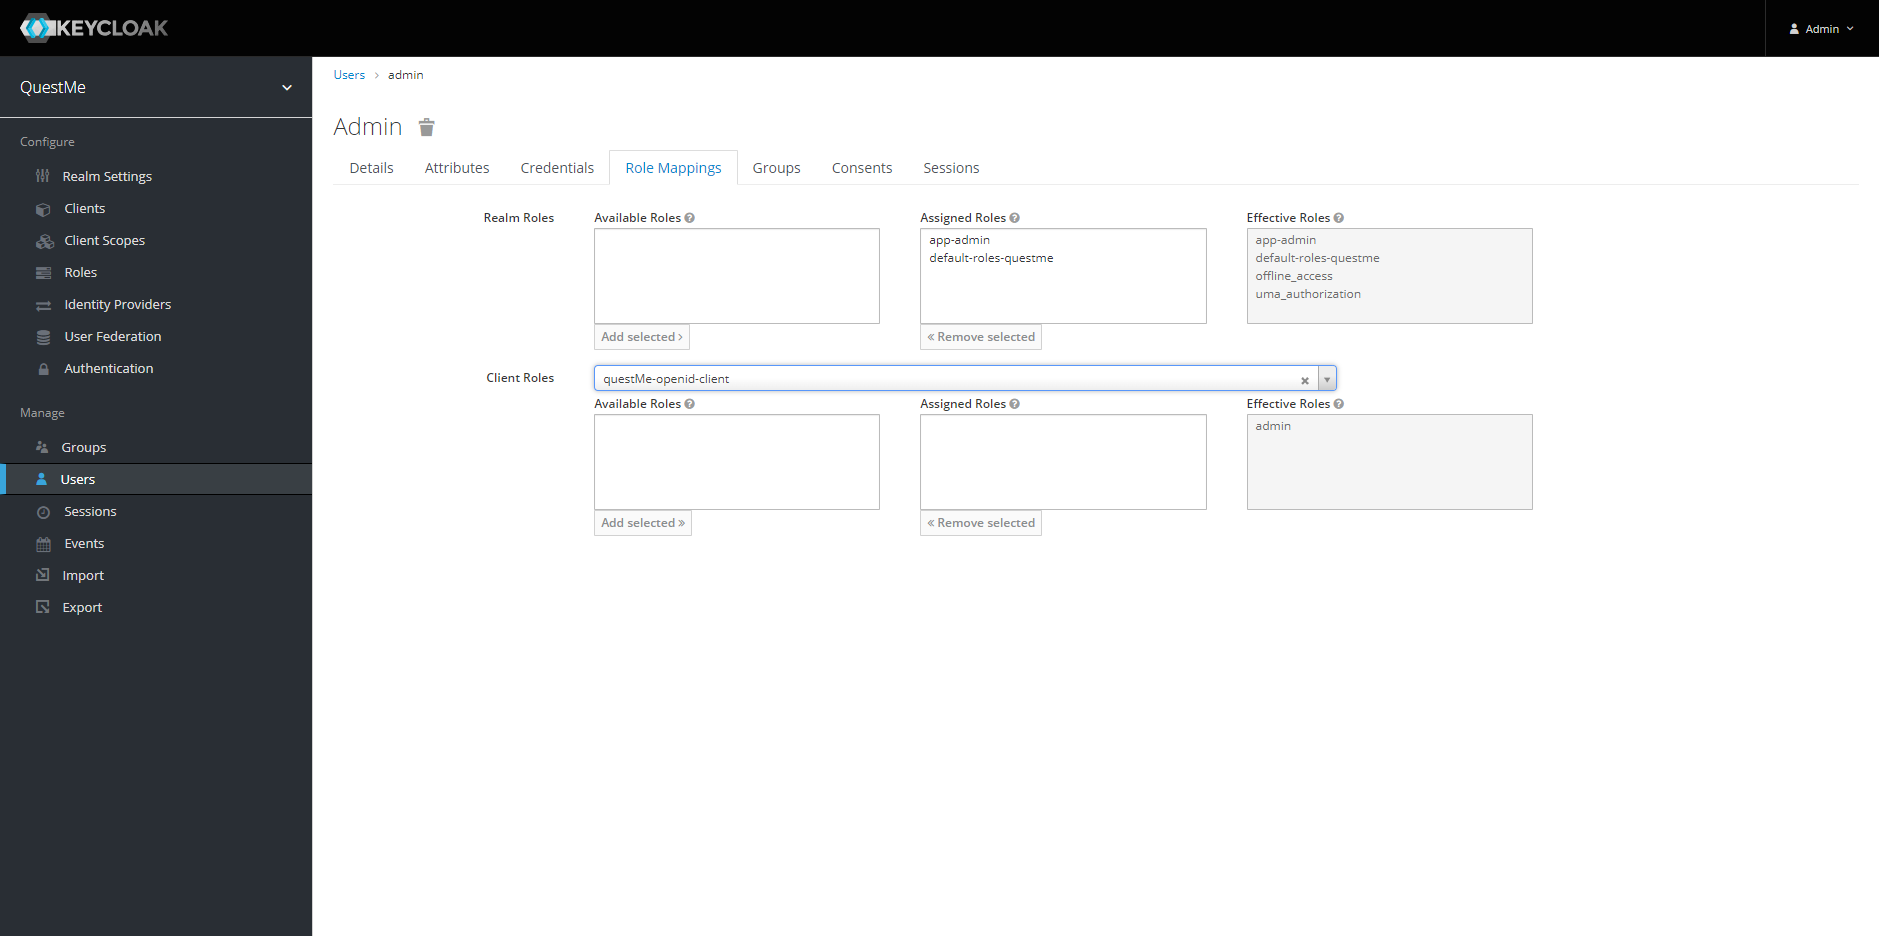
\includegraphics[width=1.0\textwidth]{bilder/administrationshandbuch/keycloak_user_roles.png}
    \caption{Keycloak User-Roles}
    \label{fig:Keycloak_User_Roles}
\end{figure}

\noindent Zum ausloggen, kann man oben rechts auf die Schaltfläche mit dem Benutzernamen ''Admin'' klicken 
und über das Dropdown-Menü ''Sign-Out'' wählen.